\documentclass[11pt,final,journal,a4paper,towside,towcolumn]{IEEEtran}
\usepackage{cite}
\usepackage{graphicx}
\usepackage[utf8]{inputenc}
\usepackage[nolist]{acronym}

\begin{document}
\begin{acronym}
	\acro{NEAT}{NeuroEvolution of Augmenting Topologies}
	\acro{KI}{Künstliche Intelligenz}
\end{acronym}
	
\title{Abschlussbericht des Team $m^2$ zu dem \\Projektpraktikum Robotik und Automation:\\Künstliche Intelligenz}
\author{Marius Krusen und F. J. Michael Werner}
\maketitle

\begin{abstract}
Brauchen wir ein Abstrakt?
\end{abstract}

\section{Aufgabenstellung}
\IEEEPARstart{Z}{iel} des Projektpraktikums ist es, eine funktionsfähige  \ac{KI} für das Spiel rAIcer zu entwickeln. In dem Spiel können bis zu drei Spieler jeweils eine Figur über mehrere Runden auf einer Rundstrecke steuern. Die Figuren werden nur durch "Kraftimpulse" in den Richtungen oben, unten, links und rechts gesteuert. In einem abschließenden Turnier, soll die \ac{KI} in der Lage sein, auf bekannten sowie unbekannten Strecken gegen \acp{KI} anderer Teams anzutreten.

\section{Lösungsansatz}
Das Team $m^2$ verwendet für die Entwicklung der \ac{KI} den \ac{NEAT}-Algorithmus. Weiterhin wird das gegebene Problem darauf reduziert, dass die \ac{KI} eine Folge von Kontrollpunkten auf der Strecke abfahren muss. Für die Berechnung der Kontrollpunkte ist eine Streckenerkennung notwendig. Für die Eingabe, der durch den \ac{NEAT}-Algorithmus generierten neuronalen Netze, werden Merkmale berechnet, die unter anderem auf den Kontrollpunkten und der Position der Figur basieren. Die einzelnen Elemente des Lösungsansatzes werden nachfolgend im Detail vorgestellt.
\subsection{NEAT}
In der Neuroevolution werden Neuronale Netze mit Hilfe von genetischen Algorithmen generiert. In \cite{stanley:gecco02-efficient} stellen Stanley et al. \ac{NEAT} vor, der die Besonderheit hat, dass neben den Kantengewichten und Schwellenwerten, auch die Topologie des Netzes entwickelt wird.
Die zentralen Bausteine des Algorithmus sind:
\begin{itemize}
\item Darstellung eines Netzes als Genom	
\item Verwendung von Historie-Markern
\item Verwendung von Spezies
\item Minimierung der Dimensionalität
\end{itemize}
In jeder Generation liegt eine Menge von Genomen (Population) vor. Durch eine Fitnessfunktion, wird die Performance der einzelnen Genome bestimmt. Anschließend werden basierend auf den stärkeren Genomen mithilfe von Mutation und Kreuzungen neue Genome für die nächste Generation erzeugt. 
Für die Implementierung des Projektes wurde das Python-Package NEAT-Python \cite{python-neat} verwendet.
\subsubsection{Genetische Darstellung und Mutation}
Jedes Genom besteht aus einer Liste von Kanten-Genen. Diese referieren jeweils auf zwei Knoten-Gene, die deren Eingangs- und Ausgangsknoten darstellen. Des Weiteren enthalten die Kanten-Gene Informationen über ihre Kantengewichte, ein Aktivierungsbit und eine Innovationsnummer. 

Mutationen in \ac{NEAT} können die Kantengewichte und die Netzstruktur verändern. Die Mutation der Kantengewichte erfolgt über Entscheidung, basierend auf Wahrscheinlichkeiten, ob ein Knoten mutiert oder nicht. Die Mutation der Struktur kann auf zwei Weisen erfolgen. Zum einen kann ein einzelnes Kanten-Gen zwischen zwei bisher nicht verbunden Knoten-Genen hinzugefügt werden, zum anderen kann ein Kanten-Gen durch zwei neue Kanten-Gene und ein neues Knoten-Gen ersetzt werden. Das alte Kanten-Gen wird dabei deaktiviert. Dadurch wird ein neuer Knoten in die Netzstruktur eingefügt.
\subsubsection{Historie-Marker und Kreuzungen}
Für die Kreuzung zweier Genome muss überprüft werden, welche Gene übereinstimmen. Dafür wird bei jedem neuen Gen eine globale Innovationsnummer erhöht und diesem Gen zugewiesen. Zwei Gene, die den gleichen historischen Ursprung haben, also eine gleiche Innovationsnummer besitzen, repräsentieren die gleiche Struktur. Während der Kreuzung kann so leicht bestimmt werden, welche Gene in beiden Elterngenomen vorliegen und übernommen werden können. Gene, die nicht in beiden Elterngenomen vorkommen, werden von dem Elterngenome mit dem höheren Fitnesswert vererbt.

\subsubsection{Spezies}
Durch das Hinzufügen einer neuen Struktur wird die Fitness anfänglich reduziert. Um eine neue Innovation zu schützen und ihr Zeit zur Optimierung zu geben, unterteilt \ac{NEAT} die Population in mehrere Spezies. Eine neue Innovation konkurriert erst mit den Genomen in der jeweiligen Spezies. Erst nach eine gewissen Zeit, wird eine Auslöschung durch einen Vergleich mit der restlichen Population möglich. Die Einteilung der Population in Spezies erfolgt durch die Berechnung einer Distanz zwischen zwei Genomen $\delta$:
\begin{equation}
\delta=\frac{c_1E}{N} + \frac{c_2D}{N} + c_3\cdot \overline{W},
\end{equation}
mit der Anzahl überflüssiger Gene $E$, die Anzahl verschiedener Gene $D$ und der durchschnittlichen Differenz der Kantengewichte übereinstimmender Gene $\overline{W}$. Die Koeffizienten $c_1, c_2, c_3$ dienen zur Gewichtung der Faktoren und $N$, die Anzahl an Genen in dem größeren Genom, dient zu Normalisierung der Distanz. Jedes Genom wird mit einem zufällig ausgewählten Genom einer Spezies verglichen. Wird ein Schwellenwert $\delta_t$ unterschritten, wird das Genom der Spezies hinzugefügt.
\subsubsection{Minimierung der Dimensionalität}
\ac{NEAT} sieht vor, dass die anfängliche Population aus Netzen besteht, die keine verdeckten Knoten hat. Dadurch dass Innovationen geschützt werden, können somit möglichst kleine Netze generiert werden, da nur neue Strukturen hinzugefügt werden, wenn sie im Sinne der Fitnessfunktion Verbesserungen einbringen.

A

\subsection{Streckenerkennung und Kontrollpunkte}
Die Streckenerkennung und die Berechnung einer Art Ideallinie oder Leitlinie, die durch eine endliche Anzahl an Kontrollpunkten repräsentiert wird, beruht im Wesentlichen auf zwei Algorithmen. Mit Hilfe der Watershed-Algorithmus wird zunächst eine grobe Leitlinie erzeugt, die einen "sicheren" Verlauf entlang der Mitte der Strecke liefert. Anschließend wird diese Leitlinie durch Verwendung eines Snake-Algorithmus, der überflüssige Richtungsänderungen eliminiert und insgesamt einen kürzeren, glatteren Kurvenverlauf erzeugt, verbessert.

\subsubsection{Watershed-Algorithmus}
Um zu Beginn überhaupt ein eindeutiges, klares Bild der Strecke zu bekommen, wird ein einfaches Schwellenwertverfahren eingesetzt, dass alle Pixel mit einem Grauwert unter 10 als schwarz und alle anderen als weiß interpretiert. Um kleine Artefakte, wie den schwarzen Rand der Figur, zu entfernen wird das resultierende Binärbild durch ein \emph{Opening} (eine Erosion gefolgt von einer Dilatation) gefiltert.
Anschließend werden mit Hilfe von OpenCV \cite{opencv} die Konturen der Strecke gefunden, um den inneren Rand der Strecke vom äußeren Rand und möglichen Hindernissen auf der Strecke zu unterscheiden. Der innere Rand wird mit Label 1 markiert, der äußere Rand und Hindernisse mit Label 2. Die eigentliche Strecke erhält kein Label. Auf Basis dieser Labels wird der Watershed-Algorithmus auf einem leeren, einfarbigen Bild ausgeführt. Der Algorithmus wird nicht auf das Bild der Strecke angewendet, da ja nicht die Ränder der Strecke, sondern die Mitte der Strecke gefunden werden soll. Durch das \emph{Fluten} des Bildes ausgehend von den Labels entsteht genau in der Mitte der Strecke eine Linie, an der Label 1 und Label 2 aufeinander treffen. Dies ist die erste grobe Leitlinie, von der in regelmäßigen Abständen ein Punkt als Kontrollpunkt für die weitere Berechnung ausgewählt wird (Bild \ref{fig-watershed}).
\begin{figure}
	\centering
	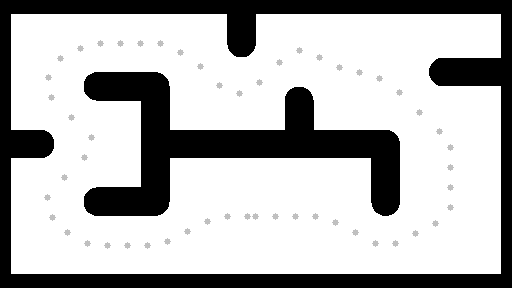
\includegraphics[width=\columnwidth]{watershed_result.png}
	\caption[Watershed-Ergebnis]{Die resultierenden Kontrollpunkte nach Anwendung des Watershed-Algorithmus}
	\label{fig-watershed}
\end{figure}

\subsubsection{Snake-Algorithmus}
Bevor der Snake-Algorithmus die Leitlinie glättet, wird der Rand der Strecke (innen, außen und Hindernisse) um den Radius der Figur dilatiert, um zu verhindern, dass der Algorithmus Kontrollpunkte liefert, die für die Figur gar nicht erreichbar sind.
Der Snake-Algorithmus (auch \emph{Aktive Kontur} genannt) beruht auf einem zu minimierendem Energieterm, der sich normalerweise aus drei einzelnen Energietermen zusammensetzt:
\begin{equation}
E = \int\alpha(s)E_{cont}(s)+\beta(s)E_{curv}(s)+\gamma(s)E_{image}ds
\end{equation}
Dabei entspricht $s$ im diskreten Fall den Punkten der Snake und $\alpha$,  $\beta$ und $\gamma$ dienen der Gewichtung der drei Terme. Der Kontinuitätsterm $E_{cont}$ dient hauptsächlich dazu, dass die Punkte der Snake einen gleichen und möglichst kurzen Abstand zueinander halten. Der Krümmungsterm $E_{curv}$ sorgt für einen glatten statt eines zackigen Kurvenverlaufs. Der Bildterm $E_{image}$ hingegen zieht die Snake zu Kanten auf dem Bild hin. Da in diesem Fall das Hauptziel eine kurze, glatte Leitlinie ist und eine zu starke Tendenz zum Rand der Strecke schädlich ist, wird auf den Bildterm verzichtet. Außerdem hat sich gezeigt, das eine gleichmäßige Gewichtung der ersten beiden Terme gute Ergebnisse liefert. Der zu minimierende Term vereinfacht sich also zu:
\begin{equation}
E = \int E_{cont}(s)+E_{curv}(s)ds
\end{equation}
Um diese Energie zu minimieren wird iterativ vorgegangen. Jeder aus dem Watershed-Algorithmus hervorgegangene Kontrollpunkt wird nacheinander betrachtet und verbessert, indem der Punkt aus dessen Nachbarschaft gesucht wird, der die Gesamtenergie am stärksten verringert. Dabei werden nur Punkte in Betracht gezogen, die auch auf der Strecke liegen. Es hat sich gezeigt, dass nach etwa 10 Durchläufen eine zufriedenstellende Leitlinie resultiert (Bild \ref{fig-snake}).
\begin{figure}
	\centering
	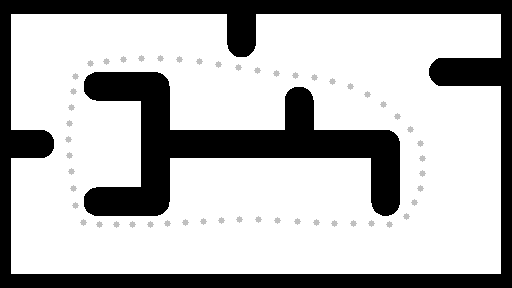
\includegraphics[width=\columnwidth]{snake_result.png}
	\caption[Snake-Ergebnis]{Die resultierenden Kontrollpunkte nach Anwendung des Snake-Algorithmus}
	\label{fig-snake}
\end{figure}

\subsection{Merkmalsberechnung}

\section{Ergebnisse}

\section{Zusammenfassung}

\bibliography{Quellen}{}
\bibliographystyle{./IEEEtranBST2/IEEEtran}
\end{document}